\begin{frame}
  \frametitle{\problemtitle}
  \begin{block}{Problem}
  	Given a point symmetric polygon, check if it can be cut into exactly two pieces of equal size along an infinite line.
  \end{block}
  \begin{center}
  	
\includegraphics[width=5cm]{sample}
  \end{center}
\end{frame}

\begin{frame}
	\frametitle{\problemtitle}
	\begin{block}{Solution}
		\begin{itemize}
			\setlength{\itemsep}{0pt}
			\item Polygon is point symmetric
			\item Parts must have equal size
			\item[] $\Longrightarrow$ Line has to go through centre of mass \textcolor{gray}{$=$ point of symmetry}
			\pause
			\item[] $\Longrightarrow$ We can do a sweepline around centre of mass
			\pause
			\item Due to symmetry, it is sufficient to keep track of the upper half of the polygon
			\pause
			\item Sweepline is valid answer $\Longleftrightarrow$ sweepline intersects the polygon exactly once
		\end{itemize}
	\end{block}
	\hspace*{\fill}
	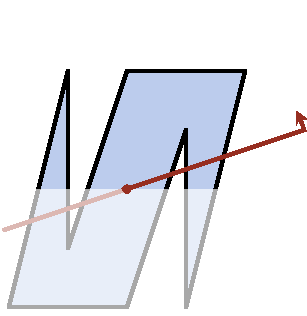
\includegraphics[width=3.5cm]{example1}
	\hspace*{\fill}
	
\includegraphics[width=3.5cm]{example2}
	\hspace*{\fill}\par
\end{frame}

\begin{frame}
	\frametitle{\problemtitle}
	\begin{block}{Sweepline}
		\begin{itemize}
			\setlength{\itemsep}{0pt}
			\item<1-> Number of intersections can only change at corners
			\item<2-> $+$ events come before $-$ events
			\item<3-> If after a type $a$ event the sweepline has size $1$, the line is ok
			\item<3-> Type $c$ events are only ok if we can rotate an $\varepsilon$ further\\
				\textcolor{gray}{(add a dummy event halfway to the next actual event)}
		\end{itemize}
	\end{block}
	\hspace*{\fill}
	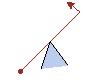
\includegraphics[width=2.5cm]{case1}
	\hspace*{\fill}
	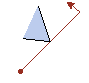
\includegraphics[width=2.5cm]{case2}
	\hspace*{\fill}
	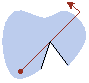
\includegraphics[width=2.5cm]{case3}
	\hspace*{\fill}
	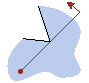
\includegraphics[width=2.5cm]{case4}
	\hspace*{\fill}\par
	
	\hspace*{\fill}
	\makebox[2.5cm]{$a$: $-2$}
	\hspace*{\fill}
	\makebox[2.5cm]{$b$: $+2$}
	\hspace*{\fill}
	\makebox[2.5cm]{$c$: $-2$}
	\hspace*{\fill}
	\makebox[2.5cm]{$d$: $+2$}
	\hspace*{\fill}
\end{frame}

\begin{frame}
	\frametitle{\problemtitle}
	\begin{block}{Edgecase}
		There might be no valid cut line that goes through any corner
	\end{block}
	\begin{center}
		\only<1>{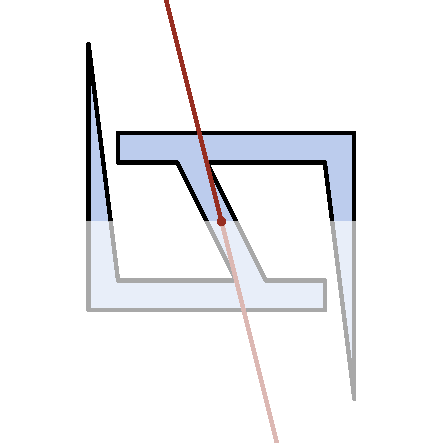
\includegraphics[width=6cm]{edgecase1}}%
		\only<2>{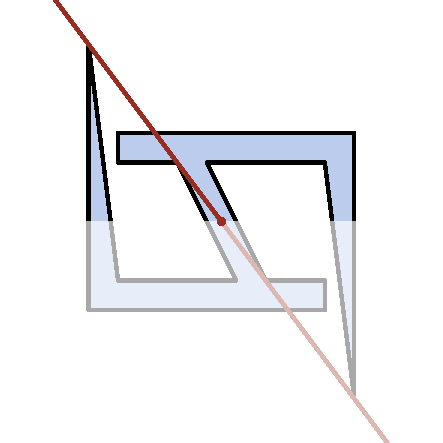
\includegraphics[width=6cm]{edgecase2}}%
		\only<3>{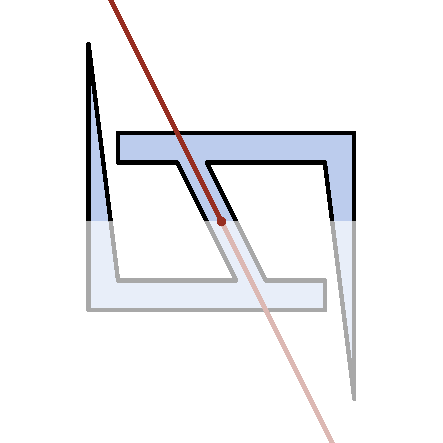
\includegraphics[width=6cm]{edgecase3}}%
	\end{center}
\end{frame}
